\documentclass[12pt]{article}
\usepackage[english]{babel}
\usepackage[utf8x]{inputenc}
\usepackage{amsmath}
\usepackage{tikz}
\usetikzlibrary{arrows,automata}
\begin{document}

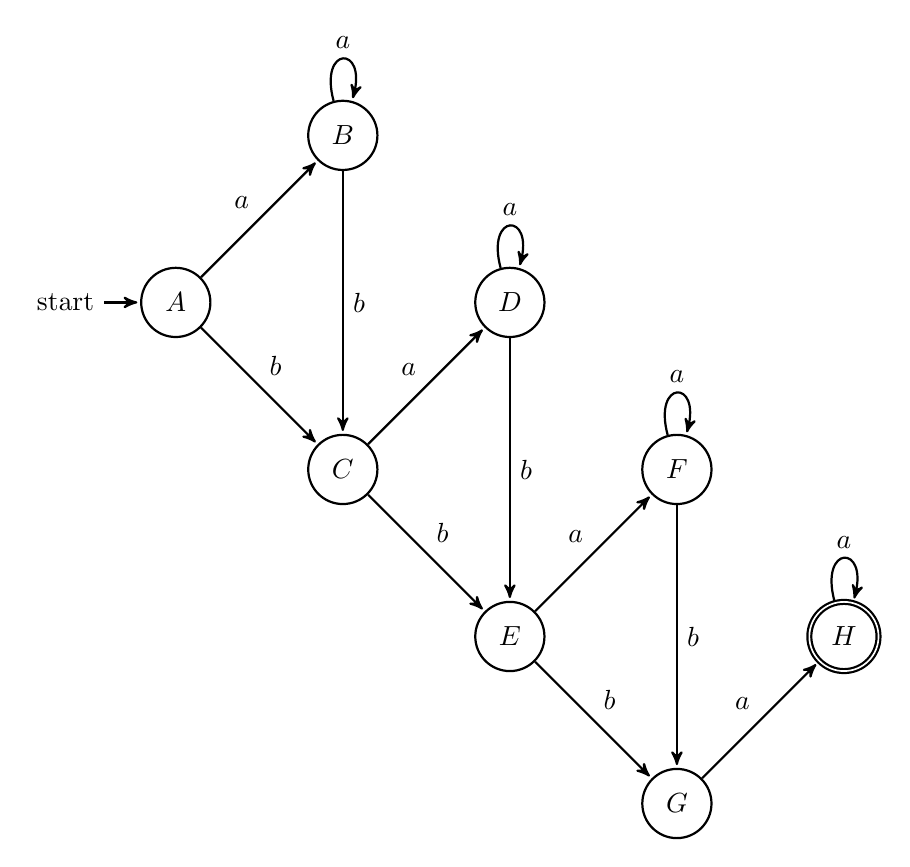
\begin{tikzpicture}[->,>=stealth',shorten >=1pt,auto,node distance=3cm,
    thick,base node/.style={circle,draw,minimum size=8pt}, real node/.style={double,circle,draw,minimum size=17pt}]

  \node[state,initial]          (a) {$A$};
  \node[state]                  (b) [above right of=a] {$B$};
  \node[state]                  (c) [below right of=a] {$C$};
  \node[state]                  (d) [above right of=c] {$D$};
  \node[state]                  (e) [below right of=c] {$E$};
  \node[state]                  (f) [above right of=e] {$F$};
  \node[state]                  (g) [below right of=e] {$G$};
  \node[state,accepting]        (h) [above right of=g] {$H$};
  \path (a) edge       node {$a$} (b)
        (a) edge       node {$b$} (c)
        (b) edge [loop above]      node {$a$} (b)
        (b) edge       node {$b$} (c)
        (c) edge       node {$a$} (d)
        (c) edge       node {$b$} (e)
        (d) edge [loop above]  node {$a$} (d)
        (d) edge       node {$b$} (e)
        (e) edge       node {$a$} (f)
        (e) edge       node {$b$} (g)
        (f) edge [loop above]  node {$a$} (g)
        (f) edge       node {$b$} (g)
        (g) edge       node {$a$} (h)
        (h) edge [loop above]     node {$a$} (h)
        
        ;

\end{tikzpicture}
\end{document}